% Options for packages loaded elsewhere
\PassOptionsToPackage{unicode}{hyperref}
\PassOptionsToPackage{hyphens}{url}
\PassOptionsToPackage{dvipsnames,svgnames,x11names}{xcolor}
%
\documentclass[
  letterpaper,
  DIV=11,
  numbers=noendperiod]{scrartcl}

\usepackage{amsmath,amssymb}
\usepackage{iftex}
\ifPDFTeX
  \usepackage[T1]{fontenc}
  \usepackage[utf8]{inputenc}
  \usepackage{textcomp} % provide euro and other symbols
\else % if luatex or xetex
  \usepackage{unicode-math}
  \defaultfontfeatures{Scale=MatchLowercase}
  \defaultfontfeatures[\rmfamily]{Ligatures=TeX,Scale=1}
\fi
\usepackage{lmodern}
\ifPDFTeX\else  
    % xetex/luatex font selection
\fi
% Use upquote if available, for straight quotes in verbatim environments
\IfFileExists{upquote.sty}{\usepackage{upquote}}{}
\IfFileExists{microtype.sty}{% use microtype if available
  \usepackage[]{microtype}
  \UseMicrotypeSet[protrusion]{basicmath} % disable protrusion for tt fonts
}{}
\makeatletter
\@ifundefined{KOMAClassName}{% if non-KOMA class
  \IfFileExists{parskip.sty}{%
    \usepackage{parskip}
  }{% else
    \setlength{\parindent}{0pt}
    \setlength{\parskip}{6pt plus 2pt minus 1pt}}
}{% if KOMA class
  \KOMAoptions{parskip=half}}
\makeatother
\usepackage{xcolor}
\setlength{\emergencystretch}{3em} % prevent overfull lines
\setcounter{secnumdepth}{-\maxdimen} % remove section numbering
% Make \paragraph and \subparagraph free-standing
\makeatletter
\ifx\paragraph\undefined\else
  \let\oldparagraph\paragraph
  \renewcommand{\paragraph}{
    \@ifstar
      \xxxParagraphStar
      \xxxParagraphNoStar
  }
  \newcommand{\xxxParagraphStar}[1]{\oldparagraph*{#1}\mbox{}}
  \newcommand{\xxxParagraphNoStar}[1]{\oldparagraph{#1}\mbox{}}
\fi
\ifx\subparagraph\undefined\else
  \let\oldsubparagraph\subparagraph
  \renewcommand{\subparagraph}{
    \@ifstar
      \xxxSubParagraphStar
      \xxxSubParagraphNoStar
  }
  \newcommand{\xxxSubParagraphStar}[1]{\oldsubparagraph*{#1}\mbox{}}
  \newcommand{\xxxSubParagraphNoStar}[1]{\oldsubparagraph{#1}\mbox{}}
\fi
\makeatother

\usepackage{color}
\usepackage{fancyvrb}
\newcommand{\VerbBar}{|}
\newcommand{\VERB}{\Verb[commandchars=\\\{\}]}
\DefineVerbatimEnvironment{Highlighting}{Verbatim}{commandchars=\\\{\}}
% Add ',fontsize=\small' for more characters per line
\usepackage{framed}
\definecolor{shadecolor}{RGB}{241,243,245}
\newenvironment{Shaded}{\begin{snugshade}}{\end{snugshade}}
\newcommand{\AlertTok}[1]{\textcolor[rgb]{0.68,0.00,0.00}{#1}}
\newcommand{\AnnotationTok}[1]{\textcolor[rgb]{0.37,0.37,0.37}{#1}}
\newcommand{\AttributeTok}[1]{\textcolor[rgb]{0.40,0.45,0.13}{#1}}
\newcommand{\BaseNTok}[1]{\textcolor[rgb]{0.68,0.00,0.00}{#1}}
\newcommand{\BuiltInTok}[1]{\textcolor[rgb]{0.00,0.23,0.31}{#1}}
\newcommand{\CharTok}[1]{\textcolor[rgb]{0.13,0.47,0.30}{#1}}
\newcommand{\CommentTok}[1]{\textcolor[rgb]{0.37,0.37,0.37}{#1}}
\newcommand{\CommentVarTok}[1]{\textcolor[rgb]{0.37,0.37,0.37}{\textit{#1}}}
\newcommand{\ConstantTok}[1]{\textcolor[rgb]{0.56,0.35,0.01}{#1}}
\newcommand{\ControlFlowTok}[1]{\textcolor[rgb]{0.00,0.23,0.31}{\textbf{#1}}}
\newcommand{\DataTypeTok}[1]{\textcolor[rgb]{0.68,0.00,0.00}{#1}}
\newcommand{\DecValTok}[1]{\textcolor[rgb]{0.68,0.00,0.00}{#1}}
\newcommand{\DocumentationTok}[1]{\textcolor[rgb]{0.37,0.37,0.37}{\textit{#1}}}
\newcommand{\ErrorTok}[1]{\textcolor[rgb]{0.68,0.00,0.00}{#1}}
\newcommand{\ExtensionTok}[1]{\textcolor[rgb]{0.00,0.23,0.31}{#1}}
\newcommand{\FloatTok}[1]{\textcolor[rgb]{0.68,0.00,0.00}{#1}}
\newcommand{\FunctionTok}[1]{\textcolor[rgb]{0.28,0.35,0.67}{#1}}
\newcommand{\ImportTok}[1]{\textcolor[rgb]{0.00,0.46,0.62}{#1}}
\newcommand{\InformationTok}[1]{\textcolor[rgb]{0.37,0.37,0.37}{#1}}
\newcommand{\KeywordTok}[1]{\textcolor[rgb]{0.00,0.23,0.31}{\textbf{#1}}}
\newcommand{\NormalTok}[1]{\textcolor[rgb]{0.00,0.23,0.31}{#1}}
\newcommand{\OperatorTok}[1]{\textcolor[rgb]{0.37,0.37,0.37}{#1}}
\newcommand{\OtherTok}[1]{\textcolor[rgb]{0.00,0.23,0.31}{#1}}
\newcommand{\PreprocessorTok}[1]{\textcolor[rgb]{0.68,0.00,0.00}{#1}}
\newcommand{\RegionMarkerTok}[1]{\textcolor[rgb]{0.00,0.23,0.31}{#1}}
\newcommand{\SpecialCharTok}[1]{\textcolor[rgb]{0.37,0.37,0.37}{#1}}
\newcommand{\SpecialStringTok}[1]{\textcolor[rgb]{0.13,0.47,0.30}{#1}}
\newcommand{\StringTok}[1]{\textcolor[rgb]{0.13,0.47,0.30}{#1}}
\newcommand{\VariableTok}[1]{\textcolor[rgb]{0.07,0.07,0.07}{#1}}
\newcommand{\VerbatimStringTok}[1]{\textcolor[rgb]{0.13,0.47,0.30}{#1}}
\newcommand{\WarningTok}[1]{\textcolor[rgb]{0.37,0.37,0.37}{\textit{#1}}}

\providecommand{\tightlist}{%
  \setlength{\itemsep}{0pt}\setlength{\parskip}{0pt}}\usepackage{longtable,booktabs,array}
\usepackage{calc} % for calculating minipage widths
% Correct order of tables after \paragraph or \subparagraph
\usepackage{etoolbox}
\makeatletter
\patchcmd\longtable{\par}{\if@noskipsec\mbox{}\fi\par}{}{}
\makeatother
% Allow footnotes in longtable head/foot
\IfFileExists{footnotehyper.sty}{\usepackage{footnotehyper}}{\usepackage{footnote}}
\makesavenoteenv{longtable}
\usepackage{graphicx}
\makeatletter
\def\maxwidth{\ifdim\Gin@nat@width>\linewidth\linewidth\else\Gin@nat@width\fi}
\def\maxheight{\ifdim\Gin@nat@height>\textheight\textheight\else\Gin@nat@height\fi}
\makeatother
% Scale images if necessary, so that they will not overflow the page
% margins by default, and it is still possible to overwrite the defaults
% using explicit options in \includegraphics[width, height, ...]{}
\setkeys{Gin}{width=\maxwidth,height=\maxheight,keepaspectratio}
% Set default figure placement to htbp
\makeatletter
\def\fps@figure{htbp}
\makeatother

\KOMAoption{captions}{tableheading}
\makeatletter
\@ifpackageloaded{caption}{}{\usepackage{caption}}
\AtBeginDocument{%
\ifdefined\contentsname
  \renewcommand*\contentsname{Table of contents}
\else
  \newcommand\contentsname{Table of contents}
\fi
\ifdefined\listfigurename
  \renewcommand*\listfigurename{List of Figures}
\else
  \newcommand\listfigurename{List of Figures}
\fi
\ifdefined\listtablename
  \renewcommand*\listtablename{List of Tables}
\else
  \newcommand\listtablename{List of Tables}
\fi
\ifdefined\figurename
  \renewcommand*\figurename{Figure}
\else
  \newcommand\figurename{Figure}
\fi
\ifdefined\tablename
  \renewcommand*\tablename{Table}
\else
  \newcommand\tablename{Table}
\fi
}
\@ifpackageloaded{float}{}{\usepackage{float}}
\floatstyle{ruled}
\@ifundefined{c@chapter}{\newfloat{codelisting}{h}{lop}}{\newfloat{codelisting}{h}{lop}[chapter]}
\floatname{codelisting}{Listing}
\newcommand*\listoflistings{\listof{codelisting}{List of Listings}}
\makeatother
\makeatletter
\makeatother
\makeatletter
\@ifpackageloaded{caption}{}{\usepackage{caption}}
\@ifpackageloaded{subcaption}{}{\usepackage{subcaption}}
\makeatother

\ifLuaTeX
  \usepackage{selnolig}  % disable illegal ligatures
\fi
\usepackage{bookmark}

\IfFileExists{xurl.sty}{\usepackage{xurl}}{} % add URL line breaks if available
\urlstyle{same} % disable monospaced font for URLs
\hypersetup{
  pdftitle={Statistical Thinking Week 2 Homework},
  colorlinks=true,
  linkcolor={blue},
  filecolor={Maroon},
  citecolor={Blue},
  urlcolor={Blue},
  pdfcreator={LaTeX via pandoc}}


\title{Statistical Thinking Week 2 Homework}
\author{}
\date{}

\begin{document}
\maketitle


\section{Chapter 4 Questions}\label{chapter-4-questions}

\textbf{4E1.} In the model definition below, which line is the
likelihood?

\[
\begin{align}
y_i &\sim \text{Normal}(\mu, \sigma) \\
\mu &\sim \text{Normal}(0, 10) \\
\sigma &\sim \text{Exponential}(1)
\end{align}
\]

\(y_i\) represents the likelihood

\textbf{4E2.} In the model definition just above, how many parameters
are in the posterior distribution?

2 Paramters: \(\mu\) and \(\sigma\)

\textbf{4E3.} Using the model definition above, write down the
appropriate form of Bayes' theorem that includes the proper likelihood
and priors.

\[
Pr(y_i | \mu, \sigma) = \frac{Pr(\mu, \sigma | y_i )Pr(y_i)}{Pr(\mu, \sigma)}
\]

\textbf{4E4.} In the model definition below, which line is the linear
model?

\[
\begin{align}
y_i &\sim \text{Normal}(\mu, \sigma) \\
\mu &= \alpha + \beta x_i \\
\alpha &\sim \text{Normal}(0, 10) \\
\beta &\sim \text{Normal}(0, 1) \\
\sigma &\sim \text{Exponential}(1)
\end{align}
\]

The Second Line

\textbf{4E5.} In the model definition just above, how many parameters
are in the posterior distribution?

3: \(\sigma\), \(\alpha\), and \(\beta\)

\section{Week 2 Homework}\label{week-2-homework}

\textbf{1.} From the Howell1 dataset, consider only the people younger
than 13 years old. Estimate the causal association between age and
weight. Assume that age influences weight through two paths. First, age
influences height, and height influences weight. Second, age directly
influences weight through age-related changes in muscle growth and body
proportions.

Draw the DAG that represents these causal relationships. And then write
a generative simulation that takes age as an input and simulates height
and weight, obeying the relationships in the DAG.

Lets first draw the dag:

\begin{Shaded}
\begin{Highlighting}[]
\NormalTok{dagified }\OtherTok{=}\NormalTok{ ggdag}\SpecialCharTok{::}\FunctionTok{dagify}\NormalTok{(}
\NormalTok{    h }\SpecialCharTok{\textasciitilde{}}\NormalTok{ a,}
\NormalTok{    w }\SpecialCharTok{\textasciitilde{}}\NormalTok{ h,}
\NormalTok{    w }\SpecialCharTok{\textasciitilde{}}\NormalTok{ a,}
    \AttributeTok{exposure =} \StringTok{"a"}\NormalTok{,}
    \AttributeTok{outcome =} \StringTok{"w"}
\NormalTok{)}

\NormalTok{ggdag}\SpecialCharTok{::}\FunctionTok{ggdag}\NormalTok{(dagified) }\SpecialCharTok{+} \FunctionTok{theme\_void}\NormalTok{()}
\end{Highlighting}
\end{Shaded}

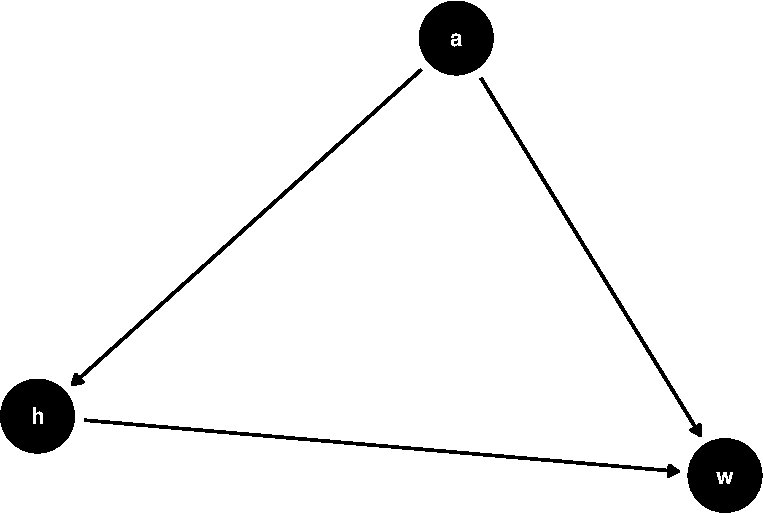
\includegraphics{week-2-homework_files/figure-pdf/unnamed-chunk-2-1.pdf}

Here is our simulation

\begin{Shaded}
\begin{Highlighting}[]
\NormalTok{sim\_weight }\OtherTok{=} \ControlFlowTok{function}\NormalTok{(A, }\AttributeTok{bAH =} \DecValTok{5}\NormalTok{, }\AttributeTok{bAW =} \FloatTok{0.5}\NormalTok{, }\AttributeTok{bHW =} \FloatTok{0.1}\NormalTok{) \{}
\NormalTok{    n }\OtherTok{=} \FunctionTok{length}\NormalTok{(A)}
\NormalTok{    H }\OtherTok{=} \FunctionTok{rnorm}\NormalTok{(n, bAH}\SpecialCharTok{*}\NormalTok{A, }\DecValTok{2}\NormalTok{)}
\NormalTok{    W }\OtherTok{=} \FunctionTok{rnorm}\NormalTok{(n, bAW}\SpecialCharTok{*}\NormalTok{A}\SpecialCharTok{+}\NormalTok{bHW}\SpecialCharTok{*}\NormalTok{H, }\DecValTok{2}\NormalTok{)}
    \FunctionTok{tibble}\NormalTok{(}\AttributeTok{Age =}\NormalTok{ A, }\AttributeTok{Height =}\NormalTok{ H, }\AttributeTok{Weight =}\NormalTok{ W)}
\NormalTok{\}}

\NormalTok{sim\_data }\OtherTok{=} \FunctionTok{sim\_weight}\NormalTok{(}\FunctionTok{runif}\NormalTok{(}\DecValTok{20}\NormalTok{, }\DecValTok{1}\NormalTok{, }\DecValTok{12}\NormalTok{))}
\NormalTok{sim\_data}
\end{Highlighting}
\end{Shaded}

\begin{verbatim}
# A tibble: 20 x 3
     Age Height Weight
   <dbl>  <dbl>  <dbl>
 1  9.32  45.1  12.4  
 2  4.31  22.5   6.12 
 3  8.08  40.0   9.31 
 4  1.65   9.43  0.750
 5 10.0   48.5   6.50 
 6  5.44  23.5   4.42 
 7  4.61  23.6   8.16 
 8  7.49  34.5   3.72 
 9  4.17  19.0   2.22 
10  8.77  43.8   7.73 
11  5.08  28.9   3.69 
12  7.74  36.5   4.96 
13  1.07   2.22  2.22 
14  9.81  47.2   9.27 
15  8.36  42.2  10.6  
16  7.82  35.3   8.23 
17  4.44  21.2   6.52 
18 10.8   49.3   8.58 
19  5.03  24.4   5.08 
20  7.97  42.9   6.39 
\end{verbatim}

\begin{Shaded}
\begin{Highlighting}[]
\NormalTok{sim\_data }\SpecialCharTok{\%\textgreater{}\%}
    \FunctionTok{ggplot}\NormalTok{() }\SpecialCharTok{+}
    \FunctionTok{geom\_point}\NormalTok{(}\AttributeTok{mapping =} \FunctionTok{aes}\NormalTok{(}\AttributeTok{x =}\NormalTok{ Age, }\AttributeTok{y =}\NormalTok{ Height))}
\end{Highlighting}
\end{Shaded}

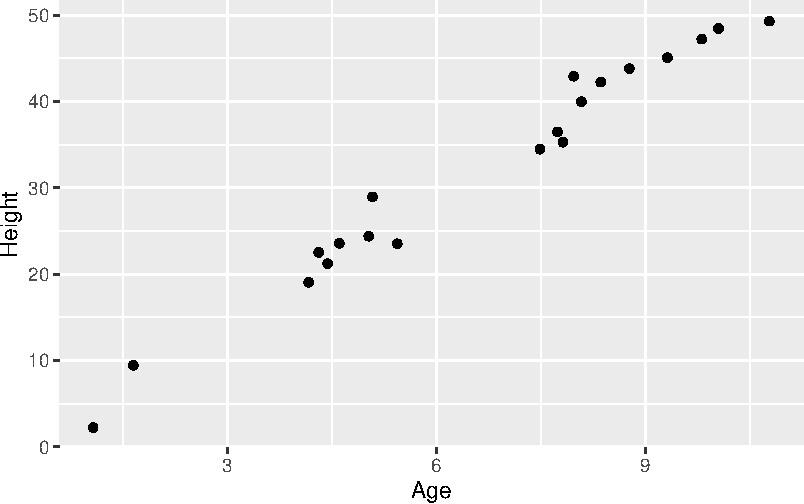
\includegraphics{week-2-homework_files/figure-pdf/unnamed-chunk-5-1.pdf}

\begin{Shaded}
\begin{Highlighting}[]
\NormalTok{sim\_data }\SpecialCharTok{\%\textgreater{}\%} 
    \FunctionTok{ggplot}\NormalTok{() }\SpecialCharTok{+}
    \FunctionTok{geom\_point}\NormalTok{(}\AttributeTok{mapping =} \FunctionTok{aes}\NormalTok{(}\AttributeTok{x =}\NormalTok{ Age, }\AttributeTok{y =}\NormalTok{ Weight))}
\end{Highlighting}
\end{Shaded}

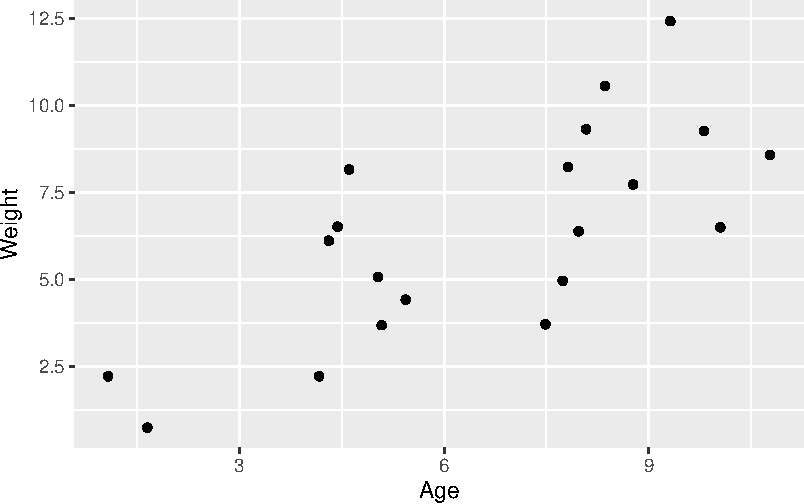
\includegraphics{week-2-homework_files/figure-pdf/unnamed-chunk-6-1.pdf}

\begin{Shaded}
\begin{Highlighting}[]
\NormalTok{sim\_data }\SpecialCharTok{\%\textgreater{}\%} 
    \FunctionTok{ggplot}\NormalTok{() }\SpecialCharTok{+}
    \FunctionTok{geom\_point}\NormalTok{(}\AttributeTok{mapping =} \FunctionTok{aes}\NormalTok{(}\AttributeTok{x =}\NormalTok{ Height, }\AttributeTok{y =}\NormalTok{ Weight))}
\end{Highlighting}
\end{Shaded}

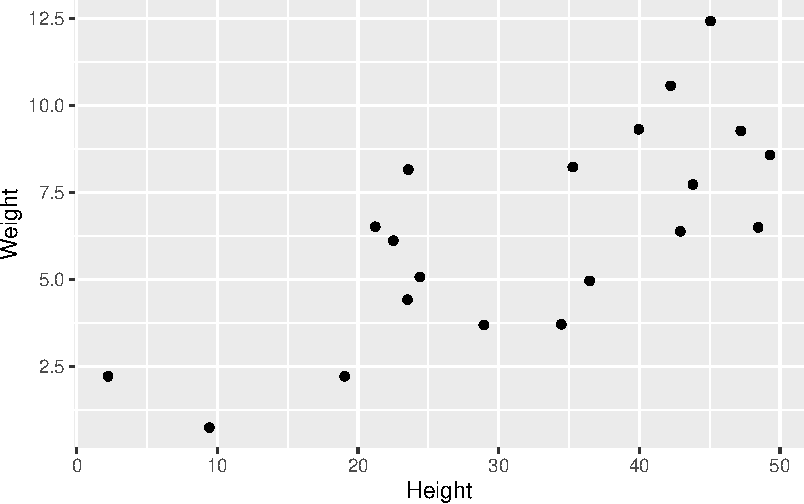
\includegraphics{week-2-homework_files/figure-pdf/unnamed-chunk-7-1.pdf}

\textbf{2.} Estimate the total causal effect of each year of growth on
weight

Lets first write our assumptions about the model. We will use similar
ones to the lecture, namely: - when age is 0, weight is 0 - As age
increases, weight increases

So lets create our model, we will assume that Age and Weight have a
linear relationship, with a gaussian distribution on error.

\[
\begin{align}
W_i &\sim \text{Normal}(\mu_i, \sigma) \\
\mu_i &= \alpha + \beta A_i \\
\alpha &\sim \text{Normal}(0, 10) \\
\beta &\sim \text{Uniform}(0, 1) \\
\sigma &\sim \text{Uniform}(0, 10)
\end{align}
\]

Using our simulation, we can generate samples

\begin{Shaded}
\begin{Highlighting}[]
\NormalTok{n }\OtherTok{=} \FloatTok{1e3}
\NormalTok{a }\OtherTok{=} \FunctionTok{rnorm}\NormalTok{(n, }\DecValTok{5}\NormalTok{, }\DecValTok{1}\NormalTok{)}
\NormalTok{b }\OtherTok{=} \FunctionTok{runif}\NormalTok{(n, }\DecValTok{0}\NormalTok{, }\DecValTok{10}\NormalTok{)}

\NormalTok{plot }\OtherTok{=} \FunctionTok{ggplot}\NormalTok{()}

\ControlFlowTok{for}\NormalTok{ (i }\ControlFlowTok{in} \DecValTok{1}\SpecialCharTok{:}\DecValTok{50}\NormalTok{) \{}
\NormalTok{    plot }\OtherTok{=}\NormalTok{ plot }\SpecialCharTok{+} \FunctionTok{geom\_abline}\NormalTok{(}\AttributeTok{slope =}\NormalTok{ b[i], }\AttributeTok{intercept =}\NormalTok{ a[i])}
\NormalTok{\}}

\NormalTok{plot }\SpecialCharTok{+} 
    \FunctionTok{scale\_x\_continuous}\NormalTok{(}\AttributeTok{limits =} \FunctionTok{c}\NormalTok{(}\DecValTok{0}\NormalTok{, }\DecValTok{14}\NormalTok{)) }\SpecialCharTok{+} 
    \FunctionTok{scale\_y\_continuous}\NormalTok{(}\AttributeTok{limits =} \FunctionTok{c}\NormalTok{(}\DecValTok{4}\NormalTok{, }\DecValTok{35}\NormalTok{))}
\end{Highlighting}
\end{Shaded}

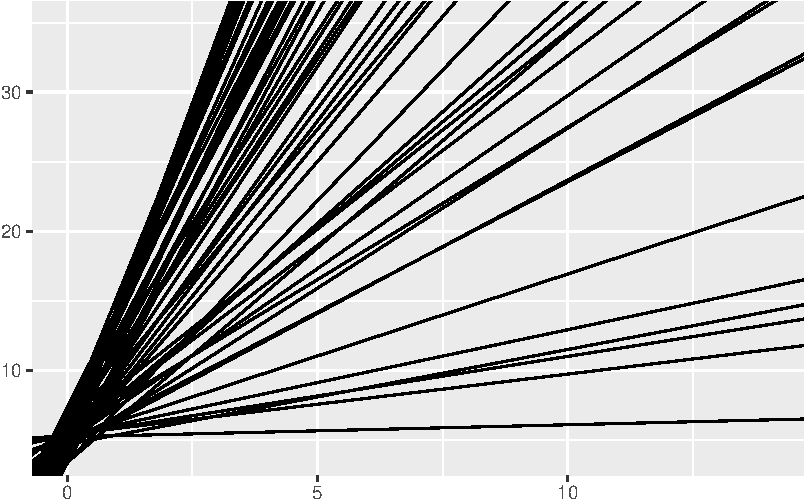
\includegraphics{week-2-homework_files/figure-pdf/unnamed-chunk-8-1.pdf}

Now lets use quadratic approximation to build a model

\begin{Shaded}
\begin{Highlighting}[]
\NormalTok{model }\OtherTok{=} \FunctionTok{quap}\NormalTok{(}
    \FunctionTok{alist}\NormalTok{(}
\NormalTok{        W }\SpecialCharTok{\textasciitilde{}} \FunctionTok{dnorm}\NormalTok{(mu, sigma),}
\NormalTok{        mu }\OtherTok{\textless{}{-}}\NormalTok{ a }\SpecialCharTok{+}\NormalTok{ b}\SpecialCharTok{*}\NormalTok{A,}
\NormalTok{        a }\SpecialCharTok{\textasciitilde{}} \FunctionTok{dnorm}\NormalTok{(}\DecValTok{5}\NormalTok{, }\DecValTok{1}\NormalTok{),}
\NormalTok{        b }\SpecialCharTok{\textasciitilde{}} \FunctionTok{dunif}\NormalTok{(}\DecValTok{0}\NormalTok{, }\DecValTok{10}\NormalTok{),}
\NormalTok{        sigma }\SpecialCharTok{\textasciitilde{}} \FunctionTok{dexp}\NormalTok{(}\DecValTok{1}\NormalTok{)}
\NormalTok{    ),}
    \AttributeTok{data =} \FunctionTok{list}\NormalTok{(}
        \AttributeTok{W =}\NormalTok{ data}\SpecialCharTok{$}\NormalTok{weight,}
        \AttributeTok{A =}\NormalTok{ data}\SpecialCharTok{$}\NormalTok{age}
\NormalTok{    )}
\NormalTok{)}

\FunctionTok{precis}\NormalTok{(model)}
\end{Highlighting}
\end{Shaded}

\begin{verbatim}
          mean         sd     5.5%    94.5%
a     7.200991 0.33293380 6.668898 7.733083
b     1.364723 0.04682846 1.289882 1.439564
sigma 2.528491 0.14146812 2.302398 2.754585
\end{verbatim}




\end{document}
